%after finding requirements more research is needed.
% Nummer, Vraag, label
\newcommand{\subquestion}[3]{
    \vspace{5mm}
    \noindent
    \textbf{Sub-question #1:} \emph{``#2''}
    \label{sq:Sub_question_#1#3}
    \newline
}
\section{Smart Home}
Main question: How does a smart home work?

\subsection{Hypothesis}
It is expected that the smart home will have multiple point of data, it centralises the data in an easy to read context so people can read the data. Data that will be found include: 
\begin{itemize}
    \item Power data of the power used in the home.
    \item Security information
    \begin{itemize}
        \item Camera images
        \item Locks
        \item Alarms
    \end{itemize}
    \item Temperature information
\end{itemize}
It will also be able to control the different equipment that is used in the house. These include:
\begin{itemize}
    \item The temperature
    \item When the lights will go on or off
    \item Timing certain uses of equipment like a dishwasher
\end{itemize}

\subsection{Sub-questions}
\begin{enumerate}
    \item What is a smart home?
    \item What are different types of smart homes?
    \item What kind of data does the smart home receive?
    \item What kind of data can the smart home control?
    \item How can the smart home be controlled?
\end{enumerate}

\subsection{Methodology}
To answer the main question the sub-questions need to be answered. To answer the sub-question it is important to explain the methods used. The methods are given below.\\
\subquestion{1}{What is a smart home?}{1}
In this chapter there will be different takes on what it means to have a smart home. It is necessary tat a look is taken at multiple research papers as to make a conclusion\\\\
\subquestion{2}{What are different types of smart homes?}{1}
To research this question smart home parts will be researched and the way it is used.\\\\
\subquestion{3}{What kind of data does the smart home receive?}{1}
This will be researched by reading papers of the possibilities and what had already been found.\\\\
\subquestion{4}{What kind of data can the smart home control?}{1}
This will be researched the same way as sub-question 2.\\\\
\subquestion{5}{How can the smart home be controlled?}{1}

\subsection{What is a smart home?}
In a research\cite{SmartHomecompare} that gives an overview of smart homes it states that:\textit{Smart home system offers people to control home environment in efficient and comfortable manner}. Another paper\cite{SmartHome_review} states that: \textit{Smart Home domain is a new trendy way of home automation and energy conservation}. A research paper\cite{SmartHomeTech} talking about the concept of the smart home states:\textit{Smart homes incorporate
common devices that control features of the home}, and that previously it was only used for environmental systems. With these three different papers it can be concluded that a smart home is a home that incorporates all common devices and control features.

\begin{figure}[H]
    \centering
    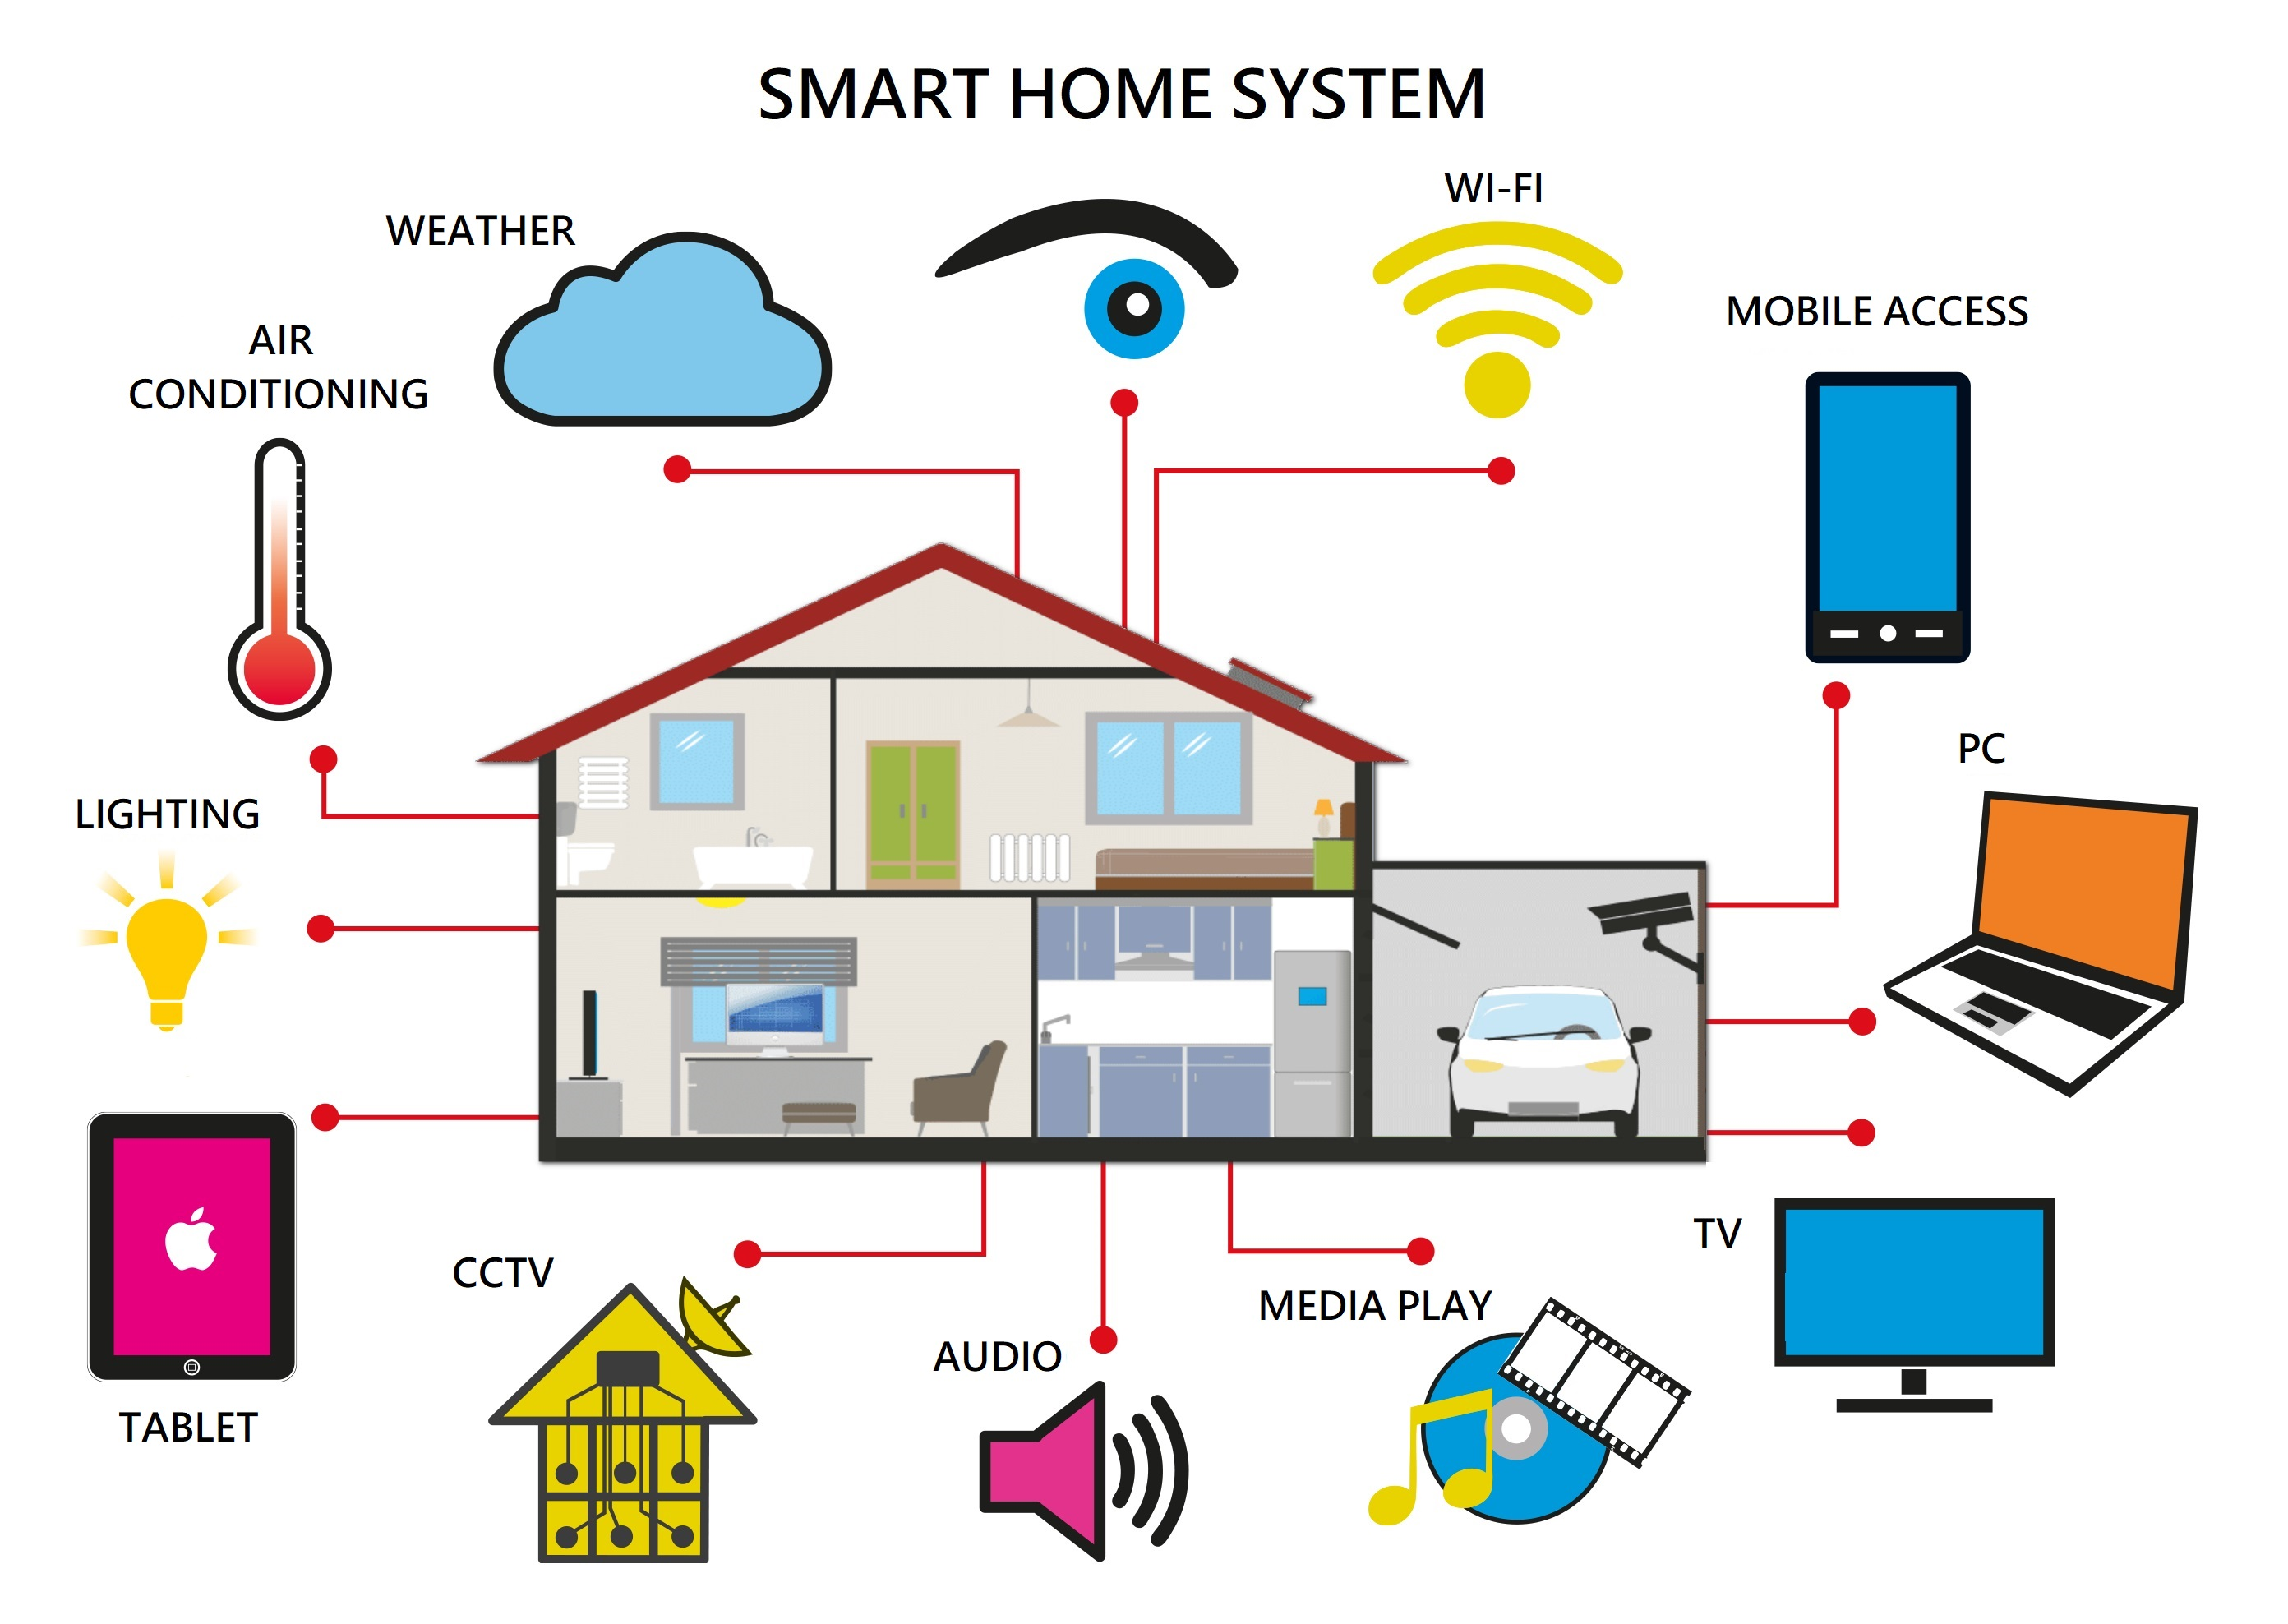
\includegraphics[width=10cm]{Images/Research/smart-home-01.jpg}
    \caption{Smart home}
    \label{fig:Smart_home}
\end{figure}

\subsection{Different types}
In a research\cite{SmartHomecompare} that compares and gives an overview of smart homes it states that there are different types of smart homes:
\begin{itemize}
    \item Dual tone multi frequency based(DTSM)
    \item Global system for mobile based(GSM)
    \item Voice recognition based
    \item Zigbee based
    \item Bluetooth based
    \item Internet and WiFi based
    \item Gesture based
\end{itemize}
The Zigbee, Bluetooth and internet and WiFi based types are all types that depend on the communication types. This entails that these smart homes use the type of communication that is stated in the name to control the devices in the house. Voice recognition is used to give commands by speaking. \\
The dual tone multi frequency based technology can make an automation system that can depict the picture of automation\cite{DualToneSH}. Which means that the DTMF can mainly be used for automating the home. This is done by using a mobile phone to automate the microcontroller\cite{SmartHomecompare}. The GSM technology also uses the mobile phone, only it uses the SMS function to command the appliances. Lastly there is gesture based which uses camera's to catch movements in order to send commands.\\

\subsection{receiving data}
\label{ss:receiving_data_research}
There is also different data that can be received. It depends on the technology used for the smart home, example given voice recognition based systems won't have the same more complicated systems connected to it that a DTSM can. So the data received will exclude gesture based and voice recognition based, because the data received isn't important. For a smart home there are two different places it can be received. These are outdoors and indoors\cite{SmartHomeTech}.
\subsubsection{Outdoors}
In the outdoors area things that can be monitored are:
\begin{itemize}
    \item Outside temperature sensor.
    \item Outside security camera's.
    \item Doorbell.
\end{itemize}
\subsubsection{Inside}
\begin{itemize}
    \item Energy usage information.
    \item Inside temperature.
    \item 
\end{itemize}

\subsection{Controlling data}
\label{ss:controlling_data_research}


\section{Router}
main question: How will the modular router be made?

\section{Sub-questions}
\begin{itemize}
    \item How big should the router be?
    \item What is the price that can be charged for the completed router?
    \item Who would use this product?
    \item How can the esp32 be used for the router?\cite{esp32_monitoring}
    \item how to flash an ESP32 board\cite{FlashingESP32}
\end{itemize}

\subsection{Methodology}
To answer the main question the sub-questions need to be answered. To answer the sub-question it is important to explain the methods used. The methods are given below. The sources for the research will mainly be searched with the google scholar search engine and Elsevier. 

\subquestion{1}{How big should the router be?}{2}
This question could be answered the best for how big routers are\\\\
\subquestion{2}{What is the price that can be charged for the completed router?}{2}
This will be done by looking at similar products that aim to have the same use.\\\\
\subquestion{3}{Who would use this product?}{2}
This can be done by asking people via a quiz or by searching for marketing stuff\\\\
\subquestion{4}{How can the esp32 be used for the router?}{2}
This is researched by searching for what the esp32 had been used before\\\\
\subquestion{5}{How to flash the esp32 board?}{2}
Looking at how people flash the esp32 and what the options are.
\\\\


\subsection{Size of the router}
In order to solve the size of the router it needs to compare different routers and see what can fit in a fuse box. 

\subsection{Price router}
This will be researched by looking at other comparable routers

\subsection{Users}
What kind of people would use the product.

\subsection{The esp32}
It is a microcontroller

\subsection{Flashing the esp32}
To flash the esp32 there are two general options. Number one is that a devkit is used and places on top of the PCB or the esp32 will be placed directly in order to flash it from one PCB. This will be cheaper and make the PCB smaller.
